\section{Limits at points}
Last time, we defined the slope of a function $ f $ by considering the `slope quotient'
\begin{equation}
  \frac{f(x + h) - f(x)}{h}.
\end{equation}
We said that a function was differentiable if we could approximate the top of this quotient by
some expression of the form $ f'(x) h $, and that the derivative of $ f $ at $ x $ was the
number $ f'(x) $.

This is a fairly intuitive definition, but there is a slight problem with it: we have no real
way of knowing which approximations are `valid'. For example, consider the function $ f(x) = x^2 $.
The top of the difference quotient becomes $ (x + h)^2 - x^2 = 2xh + h^2 $. At this point, we
wave our hands around and exclaim loudly that `because $ h $ is small, $ h^2 $ is tiny and so we
can just forget about it'. But waving our hands around is not a substitute for understanding what
is going on!

\begin{figure}
  \centering
  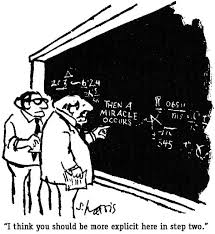
\includegraphics[width=0.3\textwidth]{handwavy}
  \caption{Let's try to be less handwavy.}
\end{figure}

This problem was rife in early discussions of calculus; the original way of dealing with it
involved talking about `infinitesimals' (this is how Leibniz thought about derivatives in the 1700s, for
example) but it turns out that this makes more problems than it solves.

The modern solution involves what are called \emph{limits}, which are a measure of how a
function behaves around a point.

\begin{defn}
  Suppose $ f(x) $ is defined for all $ x $ around a point $ a $ (but not necessarily at $ a $ itself).
  Then we say that the limit of $ f $ as $ x $ approaches $ a $ equals $ L $ if we can make the values of $ f(x) $
  as close as we like to $ L $ by taking $ x $ to be close to (but not equal to) $ a $. We write this symbolically as
  \begin{displaymath}
    \lim_{x \to a} f(x) = L,
  \end{displaymath}
  or write that $ f(x) \to L $ as $ x \to a $.
\end{defn}

The idea is that the limit of $ f $ at $ a $ is $ L $ if we can look at the graph of $ f $, cover up
the vertical line $ x = a $, and use the behaviour of $ y = f(x) $ in the neighbourhood of $ x = a $
to guess what the graph looks like at that point. \emph{The limit of $ f $ at $ a $ is dependent only
on the points around $ a $, not on the value (or lack thereof) of $ f(a) $.}

Consider the graph of a function $ g $ given in figure \ref{fig:lim1}. Although the \emph{value} of
the function at 2 is 6, the \emph{limit} of the function at 2 is $ \lim_{x \to 2} g(x) = 4 $.

\begin{figure}
  \centering
  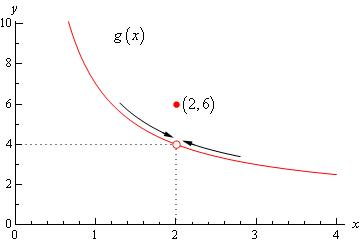
\includegraphics[width=0.4\textwidth]{oslimit2}
  \caption{A function $ g $ where $ \lim_{x \to 2} g(x) \neq g(x) $. \label{fig:lim1}}
\end{figure}

You can also think of $ \lim_{x \to a} g(x) $ as being the unique value that we could pick for $ g(a) $ such that the function
around that point has `no gaps'. If there is no such unique value, there is no limit at the point $ a $.

A function $ a $ is called \emph{continuous} at a point $ a $ if $ \lim_{x \to a} f(x) = f(a) $; that is, if it takes the
value at $ a $ which we would expect it to based on the points around $ a $. The function $ g $ graphed in figure \ref{fig:lim1}
is continuous at every point except $ x = 2 $.

Limits happen to have a few simple properties.
\begin{thm}
  If $ f $ and $ g $ are functions and the limits of $ f $ and $ g $ at $ x_0 $ exist, then:
  \begin{enumerate}
    \item $ \displaystyle \lambda \lim_{x \to x_0} f(x) = \lim_{x \to x_0} [\lambda f(x)] $ (where $ \lambda $ is a constant);
    \item $ \displaystyle \lim_{x \to x_0} f(x) + \lim_{x \to x_0} g(x) = \lim_{x \to x_0} [f(x) + g(x)] $;
    \item $ \displaystyle \left(\lim_{x \to x_0} f(x)\right)\left(\lim_{x \to x_0} g(x)\right) = \lim_{x \to x_0} [f(x)g(x)] $;
    \item $ \displaystyle \frac{\lim_{x \to x_0} f(x)}{\lim_{x \to x_0} g(x)} = \lim_{x \to x_0} \frac{f(x)}{g(x)} $ (if $ g(x) \neq 0 $ around
          the point we take the limit); and
    \item $ \displaystyle f(\lim_{x \to x_0} g(x)) = \lim_{x \to x_0} [f(g(x))] $ (if $ f $ is continuous).
  \end{enumerate}
\end{thm}

\begin{exs}
  Using these limit laws, we can find some limits reasonably easily.
  \begin{enumerate}
    \item $ \lim_{x \to 0} \frac{x}{x} = 1 $ since as $ x $ gets closer and closer to $ 0 $, $ \frac{x}{x} = 1 $.
    \item $ \lim_{x \to 3} \frac{(x - 2)(x - 3)}{x - 3} = 1 $ since as $ x $ gets closer and closer to 3, the fraction gets arbitrarily close to 1.
    \item $ \lim_{x \to 0} \frac{1}{x} $ does not exist, since if we approach 0 from the left the function becomes arbitrarily negative
          and if we approach 0 from the right the function becomes arbitrarily positive --- we do not approach the same value on both sides.
    \item $ \lim_{x \to \infty} \frac{1}{x} = 0 $ since as $ x $ becomes arbitrarily large, $ \frac{1}{x} $ becomes arbitrarily small.
    \item $ \lim_{x \to 0} \sqrt{x} $ does not exist, since $ \sqrt{x} $ is undefined for $ x < 0 $.
  \end{enumerate}
\end{exs}

\begin{figure}
  \centering
  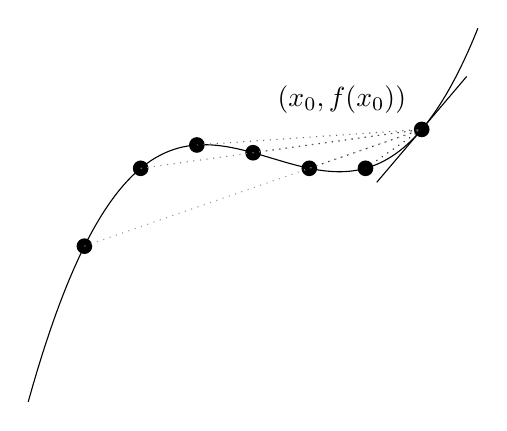
\begin{tikzpicture}
    \begin{axis}[
      axis lines = none,
      xlabel = $ x $,
      ylabel = {$ y = f(x) $}
    ] %(x -2)(x - 3) + (x + 1)(x - 3) + (x + 1)(x - 2) = x^2 - 5x + 6 + x^2 - 2x - 3 + x^2 - x - 2 = 3*16 - 2*16 + 1
      \addplot[domain = -3:5, color = black, samples = 100] {(x + 1)*(x - 2)*(x - 3) + 2};
      \node[circle,fill,inner sep=2pt] at (axis cs:-2,-18) {};
      \node[circle,fill,inner sep=2pt] at (axis cs:-1,2) {};
      \node[circle,fill,inner sep=2pt] at (axis cs:0,8) {};
      \node[circle,fill,inner sep=2pt] at (axis cs:1,6) {};
      \node[circle,fill,inner sep=2pt] at (axis cs:2,2) {};
      \node[circle,fill,inner sep=2pt] at (axis cs:3,2) {};
      \node[label={above left:{$\left(x_0,f(x_0)\right)$}},circle,fill,inner sep=2pt] at (axis cs:4,12) {};
      \draw[color=black!40, style=dotted] (-2,-18) -- (4,12);
      \draw[color=black!50, style=dotted] (-1,2) -- (4,12);
      \draw[color=black!60, style=dotted] (0,8) -- (4,12);
      \draw[color=black!70, style=dotted] (1,6) -- (4,12);
      \draw[color=black!80, style=dotted] (2,2) -- (4,12);
      \draw[color=black!90, style=dotted] (3,2) -- (4,12);
      \addplot[domain = 3.2:4.8, color=black]{12 + (x - 4)*17};
    \end{axis}
  \end{tikzpicture}
  \caption{The tangent line as a limit of secant lines.\label{fig:secants}}
\end{figure}

We will now use limits to define derivatives in a way that is relatively easier to deal with. If $ f $ is a function,
and we want to find the derivative at a point $ (x_0, f(x_0)) $, then we consider the slopes of the lines joining
this point to other points $ (x_0, f(x_0 + h)) $. As $ h \to 0 $, these secant lines become closer and closer to being
tangent lines at $ x_0 $; so if the limit of the slopes of the secant lines exist, it makes sense to define this as
the derivative $ f'(x_0) $. In other words,
\begin{equation}\label{eqn:realderivative}
  f'(x_0) = \lim_{h \to 0} \frac{f(x + h) - f(x)}{h}.
\end{equation}
See figure \ref{fig:secants} for a visualisation of this.

Just to bring ourselves back to our original formulation of derivatives as ways of computing linear
approximations, we will say that $ f(x + h) - f(x) \approx mh $ if $ f(x + h) - f(x) = mh + \vartheta(h) $,
where $ \vartheta $ is some function such that $ \vartheta(h)/h \to 0 $ as $ h \to 0 $. (To see that
this is the same thing as \ref{eqn:realderivative}, divide through by $ h $ and take the limit of both
sides as $ h \to 0 $.)

\begin{ex}
  We will find the derivative of $ f(x) = x^3 $ at the point $ x $ using the definition.
  \begin{align*}
    f'(x) &= \lim_{h \to 0} \frac{f(x + h) - f(x)}{h}\\
          &= \lim_{h \to 0} \frac{(x + h)^3 - x^3}{h}\\
          &= \lim_{h \to 0} \frac{x^3 + 3x^2h + 3xh^2 + h^3 - x^3}{h}\\
          &= \lim_{h \to 0} \frac{3x^2 h + 3xh^2 + h^3}{h}\\
          &= \lim_{h \to 0} 3x^2 + 3xh + h^2\\
          &= 3x^2.
  \end{align*}
\end{ex}

\subsection{Exercises and Problems}
\begin{enumerate}
  \item Consider the function $ f $ graphed below.
    \begin{center}
      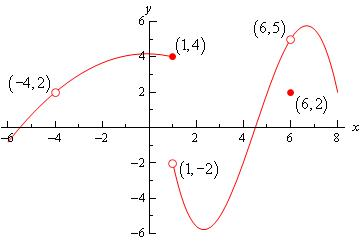
\includegraphics[width=0.4\textwidth]{oslimit}
    \end{center}
    \begin{enumerate}
      \item For each of the following expressions, either give the value or explain why the expression is undefined.
        \begin{enumerate}
          \item $ f(-4) $
          \item $ \lim_{x \to -4} f(x) $
          \item $ f(1) $
          \item $ \lim_{x \to 1} f(x) $
        \end{enumerate}
      \item Explain why the limit $ \lim_{x \to 6} f(x) $ is not equal to $ f(6) $.
      \item At which points is $ f $:
        \begin{enumerate}
          \item Discontinuous?
          \item Non-differentiable?
        \end{enumerate}
    \end{enumerate}
  \item Evaluate the limit or explain why it does not exist:
    \begin{multicols}{2}
    \begin{enumerate}
      \item $ \lim_{x \to 2} \frac{x^2 + x - 6}{x - 2} $
      \item $ \lim_{x \to 0} \frac{1}{x^3} $
      \item $ \lim_{x \to 9} \frac{1}{x^3} $
      \item $ \lim_{h \to 0} \frac{(2 + h)^3 - 8}{h} $
      \item $ \lim_{x \to 4} \frac{x^2 + 5x + 4}{x^2 + 3x - 4} $
      \item $ \lim_{x \to \frac{\pi}{2}} \sin x $
      \item $ \lim_{x \to \infty} \sin x $
      \item $ \lim_{x \to \frac{\pi}{2}} \tan x $
      \item $ \lim_{x \to 0} \tan x $
      \item $ \lim_{x \to 0} \csc x $
      \item $ \lim_{x \to a} C $, where $ a $ and $ C $ are constants.
      \item $ \lim_{x \to -\infty} \tan^{-1} x $
      \item $ \lim_{y \to 0} \lim_{x \to 0} \frac{(x + y)(x - y)}{x^2 - y^2} $
      \item $ \lim_{x \to \infty} 1/x $.
      \item $ \lim_{x \to \infty} \frac{2x}{x^2 + 1} $.
      \item $ \lim_{x \to \infty} \frac{x + 2}{x - 3} $.
    \end{enumerate}
    \end{multicols}
  \item Show that $ \lim_{x \to a} \frac{f(x) - f(a)}{x - a} $ and $ \lim_{h \to 0} \frac{f(a + h) - f(a)}{h} $ are
        equivalent definitions for the derivative at the point $ a $ of some function $ f $.
  \item If $ \lim_{x \to a} [f(x) + g(x)] = 2 $ and $ \lim_{x \to a} [f(x) - g(x)] = 1 $, find $ \lim_{x \to a} f(x)g(x) $.
  \item Explain why $ \frac{x^2 + x - 6}{x - 2} \neq x - 3 $, but $ \lim_{x \to a} \frac{x^2 + x - 6}{x - 2} = \lim_{x \to a} (x - 3) $  for every $ a $.
  \item Prove that if $ f $ is differentiable at $ a $ then it is continuous at $ a $.
  \item Last year, we defined the \emph{exponent} $ a^r $ as follows:
        \begin{itemize}
          \item If $ r = 0 $, then $ a^r = 1 $.
          \item If $ r $ is a natural number, then $ a^r = a^{r - 1} \cdot r $. (So $ a^r =\underbrace{a \times \cdots \times a}_{r \text{ times}} $.)
          \item If $ r $ is a negative integer, then $ a^r = \dfrac{1}{a^{-r}} $. (Note that $ -r $ is positive.)
          \item If $ r $ is a rational number, so that $ r = p/q $ in lowest form, then $ a^r = a^{(p/q)} = \sqrt[q]{a^p} $ (where we take the positive root,
                    if a choice needs to be made).
        \end{itemize}
        Give a reasonable definition for $ a^r $ where $ r $ is any real number. Use your definition to compute a reasonable approximation to $ 2^\pi $
        (given that $ \pi \approx 3.14159...$).
\end{enumerate}

\subsection{References}
For various exercises regarding limits, see sections 1.5 and 1.6 of Stewart. For a proper definition of limits (because the one given
above is still handwavy: what do we mean by `close'?) see Spivak (although this is beyond what the typical Y13 student needs).

For a very nice treatment of derivatives that defines $ f'(x) $ to be the unique value for $ m $ satisfying $ f(x + h) - f(x) = mh + \vartheta(h) $,
see Loomis and Sternberg, sections 3.5 and 3.6. We will use the notation $ f(x + h) \approx f'(x) h + f(x) $ in this kind of way repeatedly
for the next few sections, but won't stop to make it too rigorous; in order to do so, replace it with the equivalent equality involving $ \vartheta(h) $
and remember that $ \vartheta(h)/h \to 0 $ as $ h \to 0 $ by definition. (L \& S calls functions like $ \vartheta $ the `little-oh' class of infinitesimals.)

\subsection{Homework}
\paragraph{Reading}
The notion of limits is incredibly fundamental to mathematics. In fact, the difference between the rational numbers and the real
numbers is that, in the real numbers, every function which should have a limit at a point does have a limit at that point.

What do I mean by this?

Well, consider $ f(x) = \sqrt{x} $. Clearly we want this function to be continuous. If we apply $ f $ to the sequence
\begin{displaymath}
  x_0 = \frac{1^2}{1^2}, x_1 = \frac{14^2}{10^2}, x_2 = \frac{141^2}{100^2}, x_3 = \frac{14142^2}{1000^2}, ..., x_n = \frac{\lfloor 10^n \sqrt{2} \rfloor}{10^n}, ...
\end{displaymath}
(where $ \lfloor x \rfloor $ is the largest integer not larger than $ x $) then each output is a rational number: $ f(x_1) = 14/10 $,
for example. Furthermore, these outputs get closer and closer together so $ \lim_{n \to \infty} f(x_n) $ should exist. But the limit
cannot exist in the rationals, because $ \lim_{n \to \infty} f(x_n) = \sqrt{2} $, which is not rational!

Formally, the way we get from the rational numbers (the numbers of the form $ a/b $, where $ a $ and $ b $ are integers)
to the real numbers is by taking the set of rationals and adding to it all the limits of Cauchy sequences --- sequences
where the adjacent terms get arbitrarily close together as we walk further along them.

\paragraph{Problems}
Derivatives and limits allow us to classify functions and their behaviour. Consider the following geometric properties:
\begin{itemize}
  \item A function is \emph{increasing} if its derivative is positive.
  \item A function is \emph{decreasing} if its derivative is negative.
  \item A function is \emph{concave down} if its derivative is decreasing.
  \item A function is \emph{concave up} if its derivative is increasing.
  \item A function $ f $ is \emph{continuous} at a point $ a $ if $ \lim_{x \to a} f(x) = f(a) $.
\end{itemize}
\begin{enumerate}
  \item Describe all the function properties given above geometrically, and give an example of each.
  \item Consider the function graphed below.
        \begin{center}
          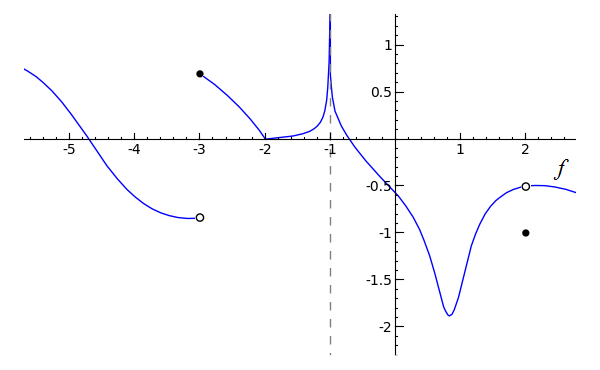
\includegraphics[width=0.5\textwidth]{limits3}
        \end{center}
    \begin{enumerate}
      \item Find $ \lim_{x \to -2} f(x) $ and $ \lim_{x \to 2} f(x) $.
      \item Does $ \lim_{x \to -3} f(x) $ exist? Why/why not?
      \item Does $ \lim_{x \to 0} f(x) $ exist? Why/why not?
      \item On what intervals is $ f(x) $ continuous?
      \item At what points is $ f(x) $ not differentiable?
    \end{enumerate}
  \item On an axis, sketch a graph of some function $ f $ that has the following features:
    \begin{itemize}[noitemsep]
      \item Is continuous for $ 0 < x < 5 $ and $ 5 < x < 9 $ and is discontinuous when $ x = 5 $
      \item Is concave down ($f''(x) < 0 $) for $ 0 < x < 5 $
      \item Has $ f'(x) = 0 $ at $ (3, 8) $
      \item Has $ \lim_{x \to 5} f(x) = 6 $.
      \item Is not differentiable at $ (7, 3) $.
    \end{itemize}
\end{enumerate}
